\section{Two NLG Tasks}
\label{sec:domains}

We begin by considering two specific NLG problems: sentence generation in the
sense of \citet{KolSto07}, and the generation of instructions in virtual
environments \citep{ByrKolStrCasDalMooObe09}. In each case, we introduce the
task and show by example how it can be viewed as a planning problem.


\subsection{Sentence generation as planning}
\label{sec:domain-crisp}

One way of modelling the sentence generation problem is to assume a
lexicalized grammar in which each lexicon entry specifies how it can
be combined grammatically with the other lexicon entries, what piece
of meaning it expresses, and what the pragmatic conditions on using it
are. Sentence generation can then be seen as constructing a
grammatical derivation that is syntactically complete, respects the
semantic and pragmatic conditions, and achieves all the
\emph{communicative goals}.

An example of such a lexicalized grammar is the tree-adjoining grammar
(TAG; \citealt{joshi;etal1997}) shown in
Figure~\ref{fig:white-rabbit-sleeps-grammar}. This grammar consists of
\emph{elementary trees} (i.e., the disjoint trees in the figure), each of
which contributes certain \emph{semantic content}. For instance, say that a
knowledge base contains the individuals $e$, $r_1$ and $r_2$, and the facts
that $r_1$ and $r_2$ are rabbits, $r_1$ is white and $r_2$ is brown, and
$e$ is an event in which $r_1$ sleeps. We could then construct a sentence
expressing the information $\{\mathsf{sleep}(e,r_1)\}$ by combining
instances of the elementary trees (in which the \emph{semantic roles}, such
as $\mathsf{self}$ and $\mathsf{subj}$, have been substituted by constants
from the knowledge base) into a TAG derivation as shown in
Figure~\ref{fig:white-rabbit-sleeps-deriv}. In the figure, the dashed arrow
indicates TAG's \emph{substitution} operation, which ``plugs'' an
elementary into the leaf of another tree; the dotted arrows stands for
\emph{adjunction}, which splices an elementary tree into an internal node.
We can then read the sentence ``The white rabbit sleeps'' from the
derivation. Note that the sentence ``The rabbit sleeps'' would not have
been an appropriate result, because ``the rabbit'' could refer to either
$r_1$ or $r_2$. Thus, $r_2$ remains as a \emph{distractor}, i.e., an
incorrect possible interpretation of the phrase.

\begin{figure}
  \centering
  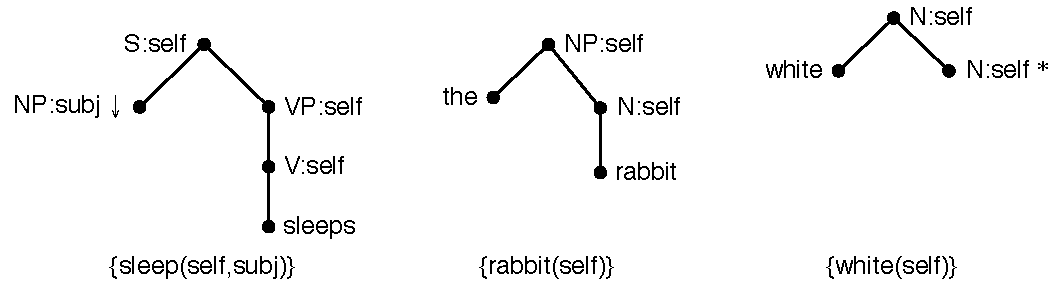
\includegraphics[width=0.75\columnwidth]{pic-grammar}
  \caption{An example grammar in the sentence generation domain.}
  \label{fig:white-rabbit-sleeps-grammar}
\end{figure}

\begin{figure}
  \centering
  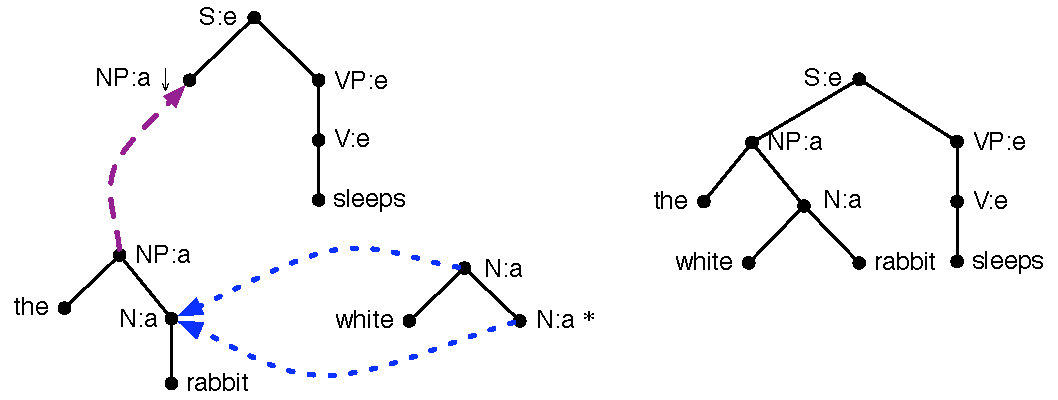
\includegraphics[width=0.75\columnwidth]{pic-derivation}
  \caption{Derivation of ``The white rabbit sleeps.''}
  \label{fig:white-rabbit-sleeps-deriv}
\end{figure}

This perspective on sentence generation also has the advantage of solving
the sentence planning and surface realization problems simultaneously,
which is particularly useful in cases where these two problems interact.
For instance, the generation of referring expressions (REs) is usually seen
as a sentence planning task, however, syntactic information about
individual words in available when the REs are generated (see, e.g.,
\citealt{stone98textual}). (In the example, we require the referring
expression ``the white rabbit'' to be resolved uniquely to $r_1$ by the
hearer, in addition to the requirement that the derivation be grammatically
correct.)


\begin{figure}
\centering
\begin{minipage}{0.8\textwidth}
{\small%
\begin{verbatim}
(:action add-sleeps
   :parameters (?u - node  ?xself - individual  ?xsubj - individual)
   :precondition
       (and (subst S ?u)  (referent ?u ?xself)  (sleep ?xself ?xsubj))
   :effect 
       (and (not (subst S ?u))  (expressed sleep ?xself ?xsubj)
            (subst NP (subj ?u))  (referent (subj ?u) ?xsubj)
            (forall (?y - individual)
                (when (not (= ?y ?xself)) (distractor (subj ?u) ?y)))))

(:action add-rabbit
   :parameters (?u - node  ?xself - individual)
   :precondition 
       (and (subst NP ?u)  (referent ?u ?xself)  (rabbit ?xself))
   :effect 
       (and (not (subst NP ?u))  (canadjoin N ?u)
            (forall (?y - individual)
                (when (not (rabbit ?y)) (not (distractor ?u ?y))))))

(:action add-white
   :parameters (?u - node  ?xself - individual)
   :precondition 
       (and (canadjoin N ?u)  (referent ?u ?xself)  (rabbit ?xself))
   :effect 
       (forall (?y - individual)
           (when (not (white ?y)) (not (distractor ?u ?y)))))
\end{verbatim}}%
\end{minipage}
\caption{PDDL actions for generating the sentence ``The white rabbit
sleeps.''}
\label{fig:white-rabbit-as-planning}
\end{figure}

However, the problem of deciding whether a given communicative goal can be
achieved with a given grammar is NP-complete \citep{KolStr02}: a naive
search algorithm that computes a derivation top-down takes exponential time
and is clearly infeasible to use in practice. In order to circumvent this
combinatorial explosion, the seminal SPUD system \citep{Stone2003a}, which
first established the idea of integrated TAG-based sentence generation,
used a greedy, but incomplete, search algorithm.
%
To better control the search, \citet{KolSto07} recently proposed an
alternative approach which converts the sentence generation problem into a
planning problem, and solves the transformed search problem using a planner
\citep{KolSto07}.\footnote{See
  \url{http://code.google.com/p/crisp-nlg/} for the CRISP system, which
  implements this conversion.} The resulting planning problem in
this case assumes an initial state containing an atom
$\mathsf{subst}(S,\mathsf{root})$, encoding the fact that a sentence ($S$)
must be generated starting at the node named $\mathsf{root}$ in the TAG
derivation tree, and a second atom $\mathsf{referent}(\mathsf{root},e)$
which encodes the fact that the entire sentence describes the (event)
individual $e$. The elementary trees in the TAG derivation are encoded as
individual planning operators.

Figure~\ref{fig:white-rabbit-as-planning} shows the
transformed planning operators needed to generate the above example
sentence, ``The white rabbit sleeps.'' Here the action instance
$\addact{sleeps}(\mathsf{root}, e, r_1)$ replaces the atom
$\mathsf{subst}(S,\mathsf{root})$ with the atom
$\mathsf{subst}(NP,\mathsf{subj}(\mathsf{root}))$. In an abuse of PDDL
syntax, we write $\mathsf{subj}(\mathsf{root})$ as a shorthand for a fresh
individual name.\footnote{These terms are not valid in
  ordinary PDDL but can be eliminated by estimating an upper bound $n$
  for the plan length, making $n$ copies of each action, ensuring that
  copy $i$ can only be applied in step $i$, and replacing the term
  $\mathsf{subj}(u)$ in an action copy by the constant
  $\mathsf{subj}_i$. The terms $S$, $NP$, and $N$ in the planning
  problem are constants.}  At the same time, the operator records that
the semantic information $\mathsf{sleep}(e,r_1)$ has now been
expressed, and introduces all individuals except $r_1$ as
distractors for the new RE at $\mathsf{subj}(\mathsf{root})$. These
distractors can then be removed by subsequent applications of the
other two operators. Eventually we reach a goal state, which is
characterized by goals including $\forall x \forall y. \neg
\mathsf{subst}(x,y)$, $\forall x \forall y. \neg
\mathsf{distractor}(x,y)$, and
$\mathsf{expressed}(\mathsf{sleep},e,r_1)$. For instance, the following
plan correctly performs the necessary derivation:
%
\begin{enumerate}
\item $\mathsf{add}\textsf{-}\mathsf{sleeps}(\mathsf{root}, r_1)$,
\todo{FIX: add-sleeps takes 3 arguments in the PDDL spec!}
\item $\mathsf{add}\textsf{-}\mathsf{rabbit}(\mathsf{subj}(\mathsf{root}),r_1)$,
\item $\mathsf{add}\textsf{-}\mathsf{white}(\mathsf{subj}(\mathsf{root}),r_1)$.
\end{enumerate}
%
The grammatical derivation in
Figure~\ref{fig:white-rabbit-sleeps-deriv}, and therefore the
generated sentence ``the white rabbit sleeps,'' can be systematically
reconstructed from this plan. Thus, we can solve the sentence
generation problem via the detour through planning and bring current
search heuristics for planning to bear on generation.


\subsection{Planning in instruction giving}
\label{sec:domain-give}

In the second application of planning in NLG, we consider the recent GIVE
Challenge (``Generating Instructions in Virtual Environments'';
\citealt{ByrKolStrCasDalMooObe09}). The object of this shared task is to
build an NLG system which produces natural language instructions which
guide a human user in performing a task in a virtual environment. From an
NLG perspective, GIVE makes for an interesting challenge since it is a
theory-neutral task that exercises all components of an NLG system, and
emphasizes the study of communication in a (simulated) physical
environment. Furthermore, because the client displaying the 3D environment
to the user can be physically separated from the NLG system (provided they
are connected over a network), such systems can be cheaply evaluated over
the Internet. This provides a potential solution to the long-standing
problem of evaluating NLG systems. The first instalment of GIVE (GIVE-1)
evaluated five NLG systems on the performance of 1143 users, making it the
largest ever NLG evaluation effort to date in terms of human users.

\begin{figure}[t]
\centering
%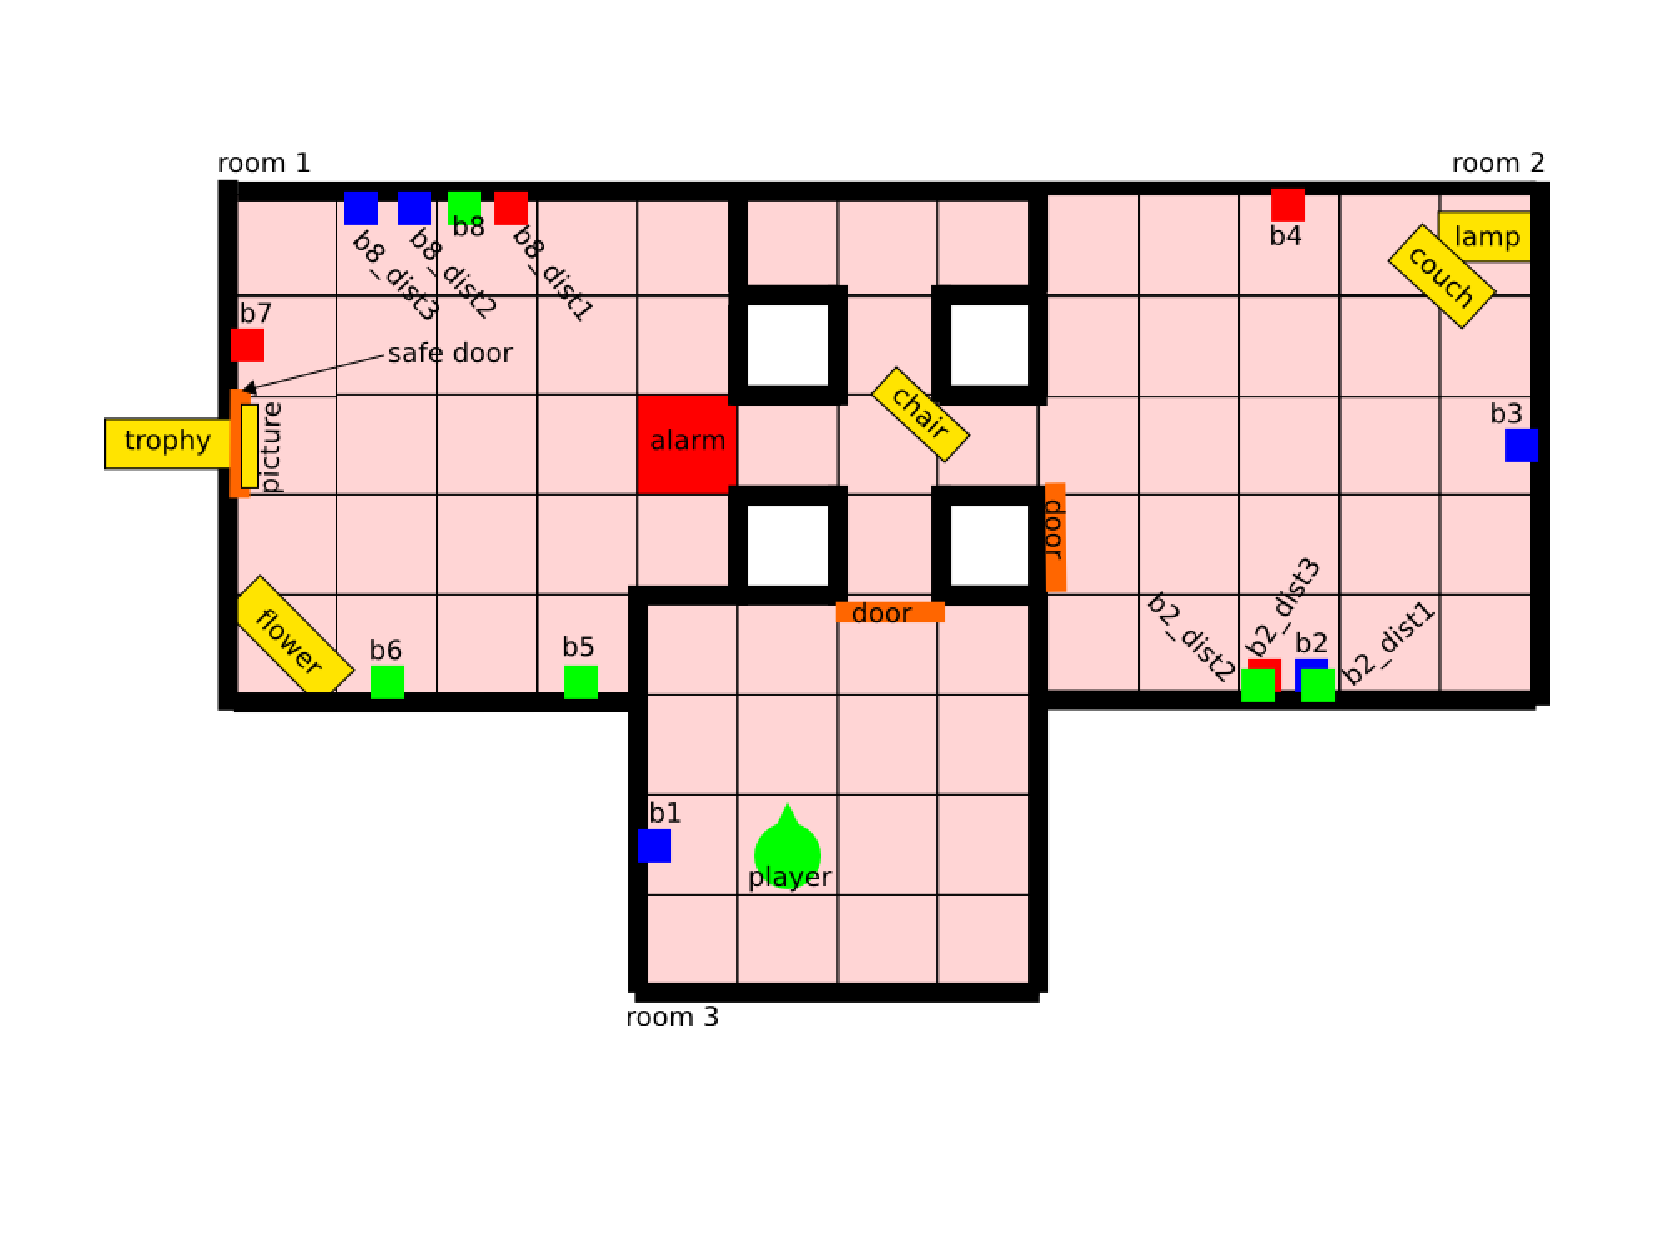
\includegraphics[width=1 \columnwidth]{give_world_no_expl}
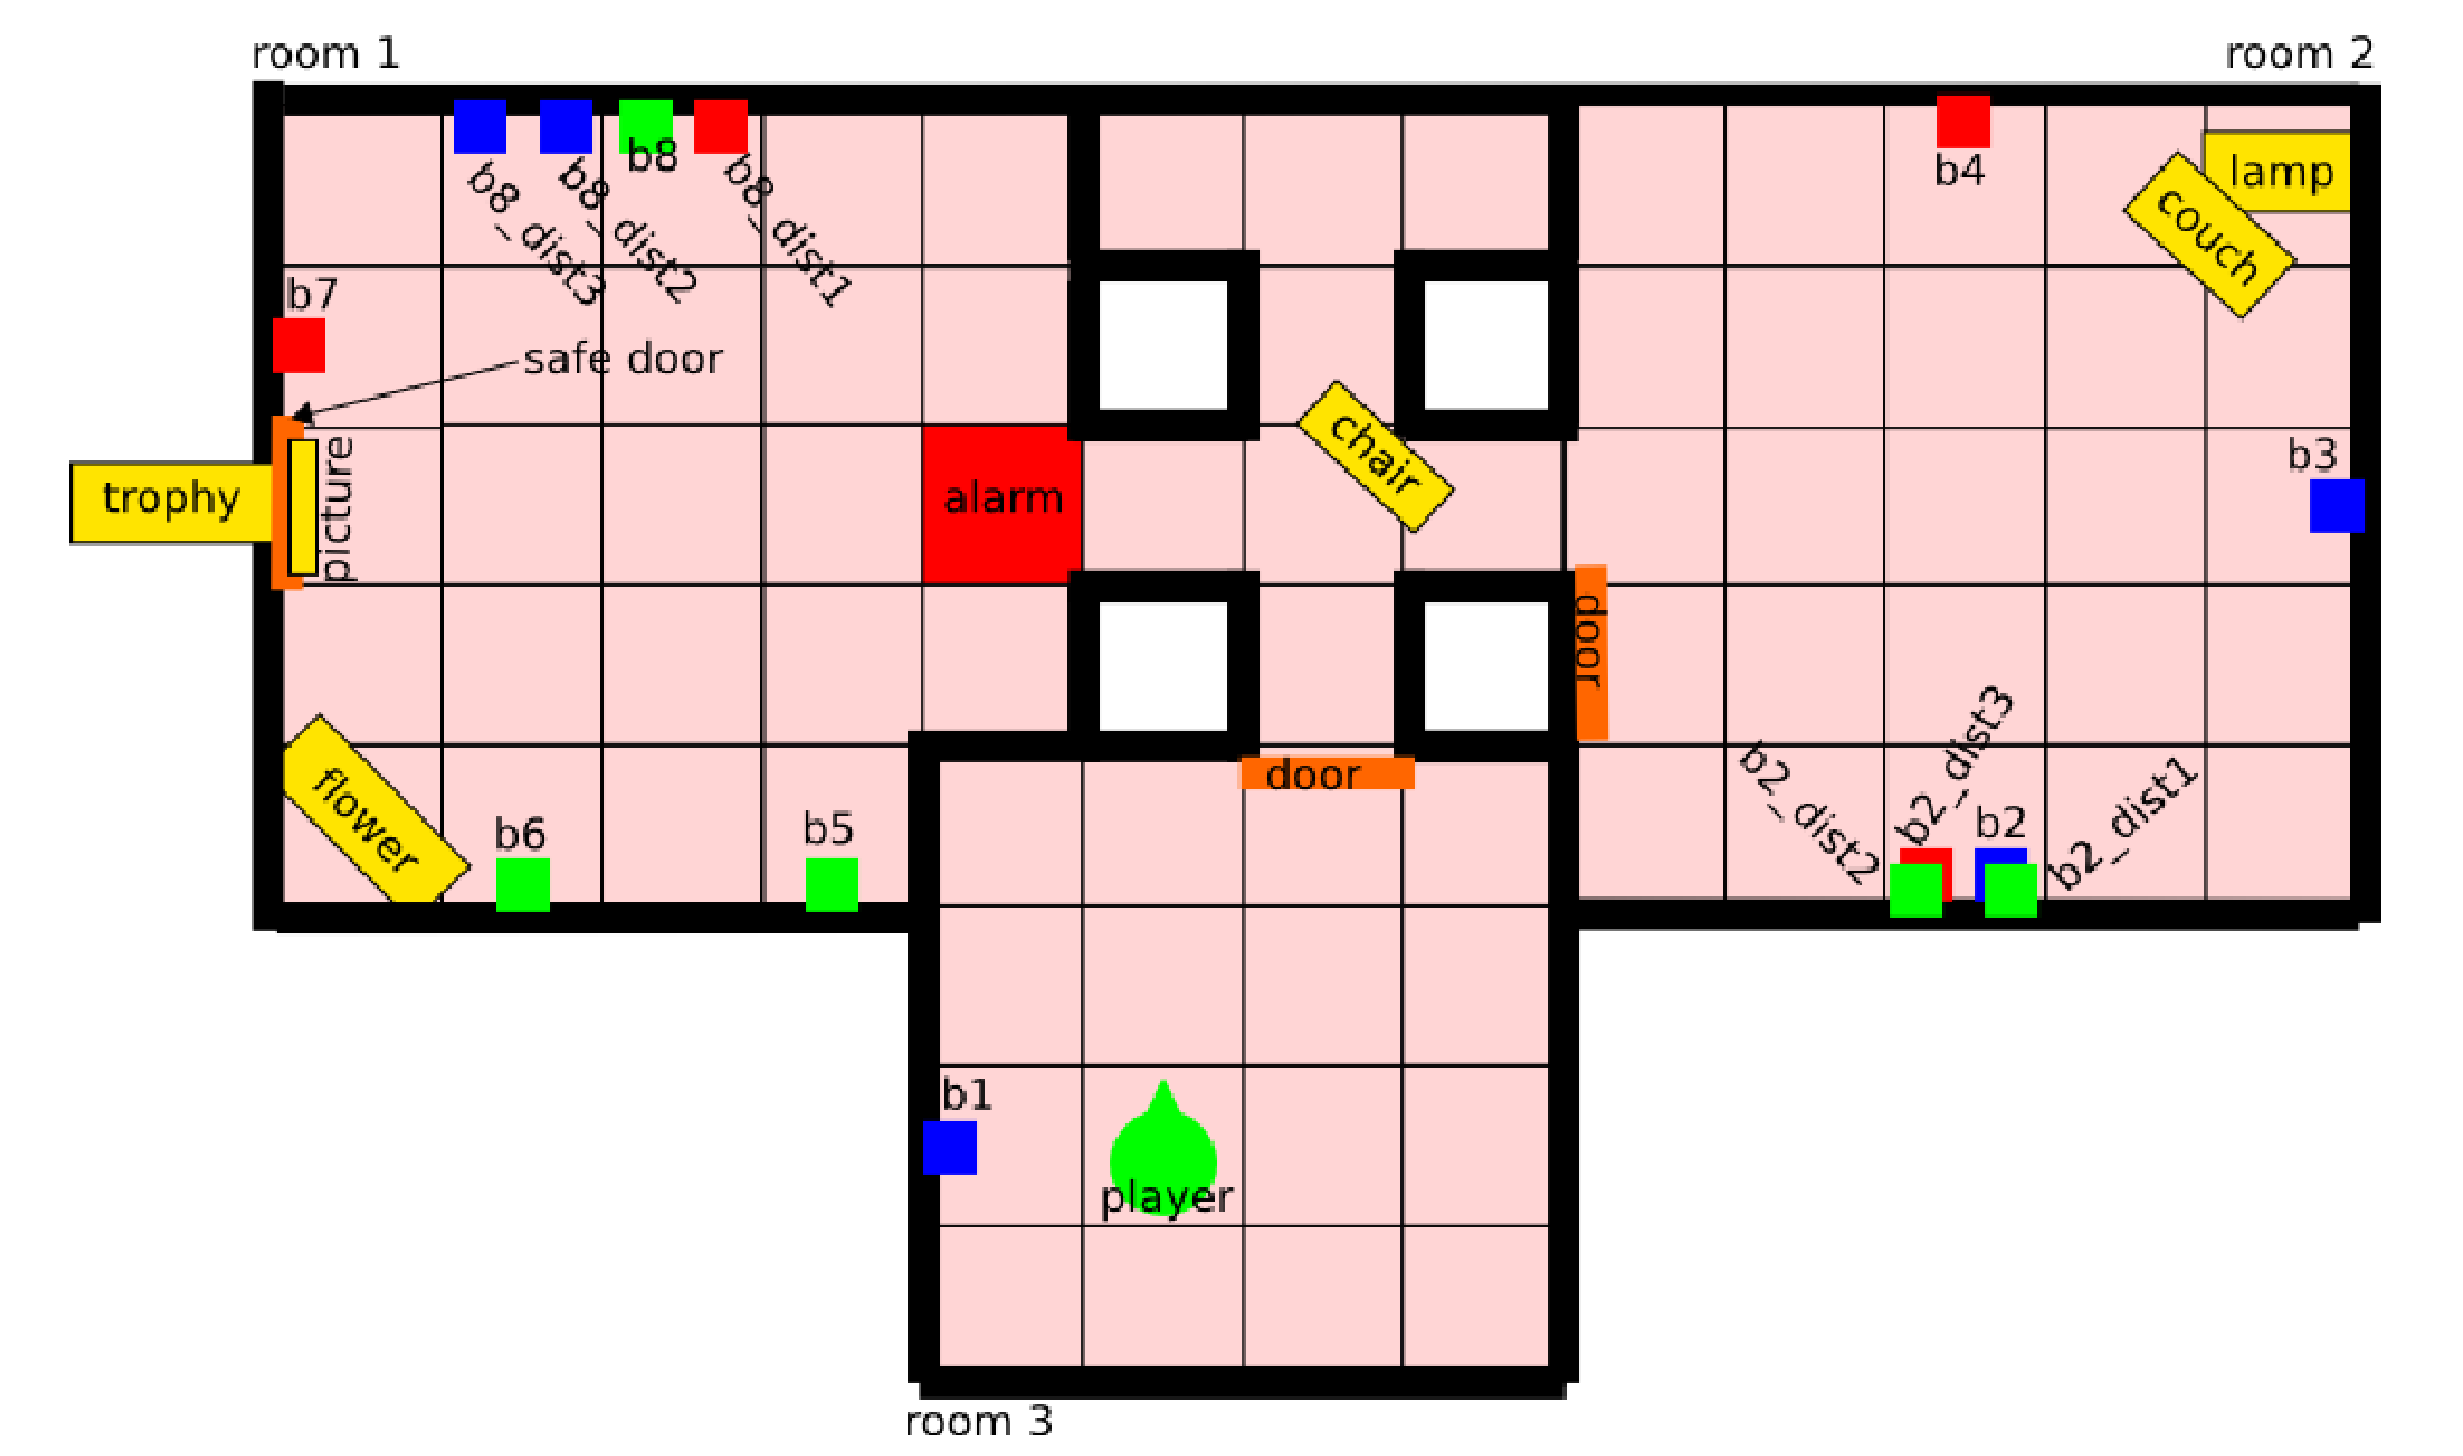
\includegraphics[width=0.75\columnwidth]{give_world_2}
\caption{Map of an example GIVE world.}
  \label{fig:give-development-world}
\end{figure}

Planning plays a central role in the GIVE task. For instance, consider the
example GIVE world shown map in Figure~\ref{fig:give-development-world}. In
this world, the user's task is to pick up a trophy in the top left room.
The trophy is hidden in a safe behind a picture; to access it, the user
must push certain buttons in order to move the picture out of the way, open
the safe, and open doors. The user must navigate the world and perform
these actions in the 3D client; the NLG system must instruct the user on
how to do this. To simplify both the planning and the NLG task, the world
is discretised into a set of tiles of equal size. The user can turn by 90
degree steps in either direction, and can move from the centre of one tile
to the centre of the next tile, provided the path between two tiles is not
blocked. Figure~\ref{fig:give-planning} shows the encoding of some of the
available GIVE domain actions in PDDL syntax. In the example, the shortest
plan to solve the task consists of 108 action steps, with the first few
steps as follows:
%
\begin{enumerate}
\item $\mathsf{turn}\textsf{-}\mathsf{left}(\mathsf{north},
\mathsf{west})$,
\item $\mathsf{move}(\mathsf{pos\_5\_2}, \mathsf{pos\_4\_2}, \mathsf{west})$,
\item $\mathsf{manipulate}\textsf{-}\mathsf{button}\textsf{-}\mathsf{off}\textsf{-}\mathsf{on}(\mathsf{b1, pos\_5\_2})$,
\item $\mathsf{turn}\textsf{-}\mathsf{right}(\mathsf{west}, \mathsf{north})$.
\end{enumerate}

\begin{figure}
\centering
\begin{minipage}{0.9\textwidth}
{\small%
\begin{verbatim}
(:action move
   :parameters (?from - position  ?to - position  ?ori - orientation)
   :precondition 
       (and (player-position ?from)  (player-orientation ?ori)
            (adjacent ?from ?to ?ori)  (not (alarmed ?to)))
   :effect 
       (and (not (player-position ?from))  (player-position ?to)))

(:action turn-left
   :parameters (?ori - orientation  ?newOri - orientation)
   :precondition 
       (and (player-orientation ?ori)  (next-orientation ?ori ?newOri))
   :effect 
       (and (not (player-orientation ?ori))  (player-orientation ?newOri)))

(:action turn-right
   :parameters (?ori - orientation  ?newOri - orientation)
   :precondition 
       (and (player-orientation ?ori)  (next-orientation ?newOri ?ori))
   :effect 
       (and (not (player-orientation ?ori))  (player-orientation ?newOri)))

(:action manipulate-button-off-on
   :parameters (?b - button  ?pos - position  ?alarm - position)
   :precondition 
       (and (state ?b off)  (player-position ?pos)  (position ?b ?pos)
            (controls-alarm ?b ?alarm))
   :effect
       (and (not (state ?b off))  (not (alarmed ?alarm))  (state ?b on)))
\end{verbatim}}%
\end{minipage}
\caption{Simplified PDDL actions for the GIVE domain.}
\label{fig:give-planning}
\end{figure}

Our description of GIVE as a planning problem makes it very similar to the
classic Gridworld problem (see, e.g., \citealt{Tovey-Koenig:2000}
or the 1998 edition of the IPC\footnote{See
\texttt{ftp://ftp.cs.yale.edu/pub/mcdermott/aipscomp-results.html}.}),
which also involves route finding through a two-dimensional world map with
discrete positions. As in Gridworld, the domain also requires the
execution of certain object-manipulation actions (e.g., finding keys and
opening locks in Gridworld, or pushing the correct buttons to open doors
and the safe in GIVE). However, the worlds we consider in GIVE tend to be
much bigger than the Gridworld instances used in the 1998 planning
competition, with more complex room shapes and more object types in the
world.

To be successful in GIVE, an NLG system must be able to compute plans of
the form described above. At a minimum, a discourse planner will call a
domain planner in order to determine the content of the instructions that
should be presented to the user. This relatively loose integration of
NLG system and planner is the state of the art of the systems that
participated in GIVE-1. However, it is generally desirable to integrate the
planner and the generation system more closely than this. For instance,
consider an NLG system that wants to generate the instruction sequence
``walk to the centre of the room; turn right; now press the green button in
front of you''. Experiments with human instruction givers \citep{stoia:08}
show that this is a pattern that they use frequently: the instruction
follower is made to walk to a certain point in the world where the
instruction giver can then use a referring expression (``the green
button'') that is easy for the follower to interpret. An NLG system must
therefore integrate discourse planning and planning in the domain of the
world map closely. On the one hand, the structure of the discourse is
determined by the needs of the NLG system rather than the domain plan; on
the other hand, the discourse planner must be aware of the way in which the
instruction ``turn right'' is likely to change the visibility of objects.
Even if an NLG system doesn't implement the generation of such discourse as
planning, it must still solve a problem that subsumes the domain planning
problem. For these reasons, we consider the GIVE domain planning problem as
a natural part of a GIVE NLG system.  

%%% Local Variables: 
%%% mode: latex
%%% TeX-master: "manuscript"
%%% End: 
